%% Fall 2013 MDM Homework Template
\documentclass[12pt,letterpaper]{article}

\usepackage[utf8]{inputenc}
\usepackage[T1]{fontenc}
\usepackage{amsmath}
\usepackage{amsfonts}
\usepackage{amssymb}
\usepackage{amsthm}
\usepackage[left=2cm,right=2cm,top=2cm,bottom=2cm,headheight=22pt]{geometry}
\usepackage{fancyhdr}
\usepackage{setspace}
\usepackage{lastpage}
\usepackage{graphicx,subcaption}

\theoremstyle{definition}
\newtheorem{task}{Task}

\begin{document}

%other parameters
\setlength{\parskip}{1ex plus 0.5ex minus 0.2ex}
\setlength{\parindent}{0pt}

%header and footer parameters
\pagestyle{fancy}
\lhead{Math 1100}
\chead{Weekly Homework}
\rhead{Due: February 5}
\lfoot{}
\cfoot{\emph{Prof. Hitchman}}
\rfoot{}

\begin{center}
{
\Large
\textbf{Knots: Written Assignment \#4}
}
\end{center}

To earn a passing mark, your assignment must:
\begin{itemize}
\item be written legibly. Diagrams may be hand drawn, but should be clear enough to read easily.
\item address the three writing prompts below.
\item conform to reasonable standards for grammar, spelling, and usage of the English language with minimal errors. (You may consider seeking help on writing from the Writing Center in the Academic Learning Center. http://www.uni.edu/unialc/writing-center)
\item be turned in by 3pm (the end of class) on Friday, February 5.
\end{itemize}




\begin{task}
Explain why the second rule for tricolorability means that the standard projection of the unknot, which is just a regular circle, is not tricolorable.
\end{task}

\begin{task}
Show that this knot is tricolorable by drawing it with a coloring scheme which satisfies the rules.
\begin{figure}[h]
\centering
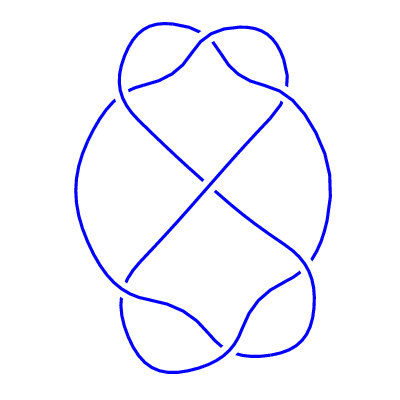
\includegraphics[width=.25\textwidth]{knotpics/7_4.png}
\caption{A tricolorable knot with seven crossings}
\end{figure}
\end{task}

%\clearpage

\begin{task}
For each of the two knots below, say whether the knot is tricolorable or not. Explain clearly, in detail, how you know.
\begin{figure}[h]
    \centering
    \begin{subfigure}{.25\textwidth}
        \centering
        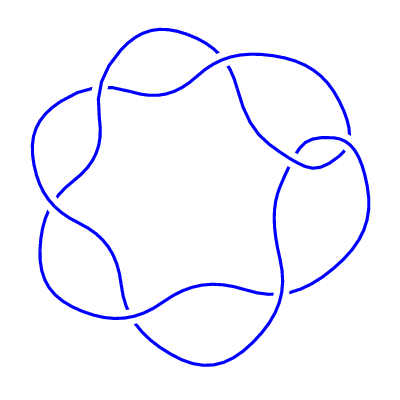
\includegraphics[width=\textwidth]{knotpics/7_2.png}
        \caption{Knot A}
    \end{subfigure}
    \qquad\qquad\qquad
    \begin{subfigure}{.25\textwidth}
        \centering
        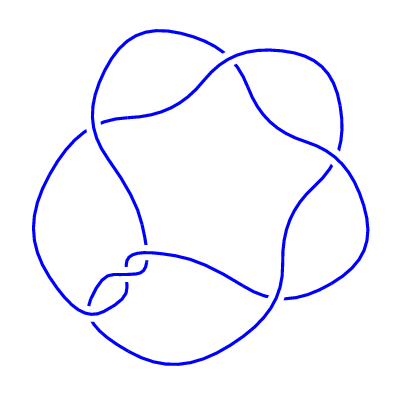
\includegraphics[width=\textwidth]{knotpics/7_3mirror.png}
        \caption{Knot B}
    \end{subfigure}
    \caption{Two knots with seven crossings}
\end{figure}
\end{task}




\end{document}
%sagemathcloud={"zoom_width":100}